\section{Descrizione delle usecases} \hypertarget{section::\theHsection}
In questa sezione andremo a schematizzare i requisiti funzionali del software da sviluppare, essi sono indipendenti dalla tipologia di tecnologia utilizzata, dall'architettura, dalla piattaforma e dalla tipo di linguaggio di programmazione scelto.

Nel nostro caso avremo un attore Utente che interagisce con il sistema, questi potrà invocare una Richiesta Percorso(UC1) che a sua volta include un altro caso d'uso che si occuperà della generazione del percorso(UC2).

Generazione percorso fa utilizzo di due API esterne: Open Street Map si occuperà di fornire una mappa del percorso (planner) mentre Open Charge Map è un database contente tutte le informazioni sulla posizione delle colonnine di ricarica.

L'Utente potrà Registrarsi(UC8) ed effettuare un Login(UC10) all'applicazione web in modo da ottenere dei Servizi Aggiuntivi(UC3).

I servizi aggiuntivi offerti sono il Salvataggio dei Luoghi Preferiti(UC4), Modifica Dati Utente(UC5), Esportare il Percorso(UC6), Generazione dei Report(UC7), Cancellazione Utente(UC9) e il Logout(UC11).
\\\\\\\\\\\\\\\\

\begin{figure}[htp]
\centering
{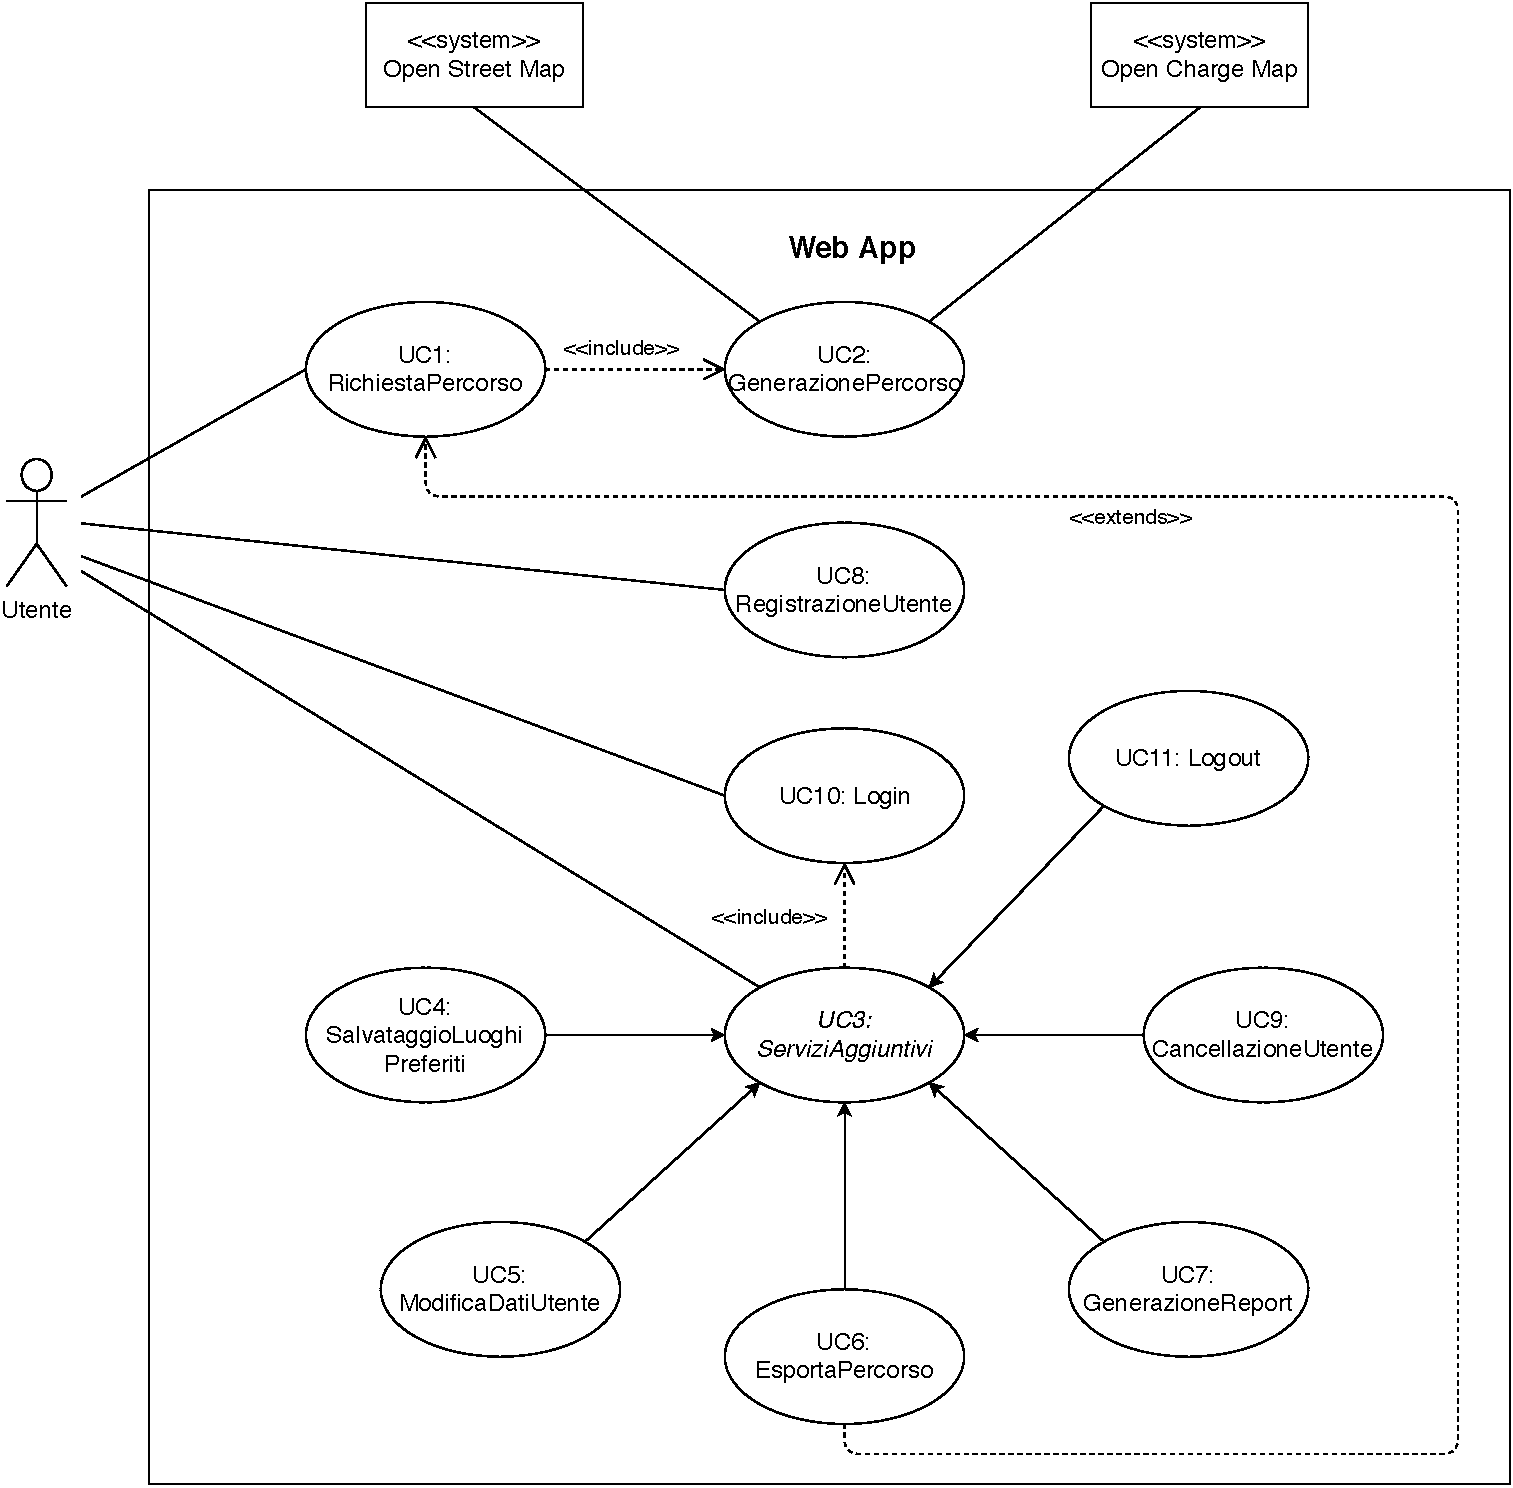
\includegraphics[scale=0.55]{Immagini/UseCases.pdf}}
\caption{Diagramma dei casi d'uso\label{t1v2}}
\end{figure}

\underline{\textbf{UC1: RichiestaPercorso}}

\begin{enumerate}
\item\textbf{Descrizione} \\ L'utente desidera ottenere il tragitto fra due località comprensivo delle soste da effettuare presso le colonnine di ricarica. %Vuole inoltre conoscere la durata della sosta presso ogni colonnina.
\item\textbf{Requisiti coperti}\\ /
\item\textbf{Attori} \\ Utente
\item\textbf{Precondizioni} \\ L'utente ha accesso alla pagina web ed è pronto ad inserire i dati richiesti
\item\textbf{Passi principali}
\begin{enumerate}
\item L'utente inserisce la località di partenza, quella di destinazione desiderata e l'autonomia dell'auto
\item Controllo che le località di inizio, fine percorso e autonomia sono inserite con la giusta formattazione 
\item Controllo che le località inserite sono valide e che l'autonomia sia stata inserita correttamente(valori negativi non ammessi)
\item Le informazioni circa le località inserite dall'utente vengono processate attraverso Open Street Map al fine di convertire gli indirizzi in coordinate
\item Le coordinate vengono inviate al modulo di analisi con il relativo campo autonomia
\end{enumerate}
\item\textbf{Situazioni eccezionali} \\ /
\item\textbf{Postcondizioni} \\ Coordinate formattate
\end{enumerate}

\underline{\textbf{UC2: GenerazionePercorso}}

\begin{enumerate}
\item\textbf{Descrizione} \\ Generazione del percorso finale comprensivo di soste per le ricariche dell'auto
\item\textbf{Requisiti coperti} \\ R1
\item\textbf{Attori} \\ /
\item\textbf{Precondizioni} \\ Coordinate formattate
\item\textbf{Passi principali}
    \begin{enumerate}
    \item Le coordinate ricevute vengono fornite a Open Street Map per ottenere il percorso fra i due punti
    \item Il percorso ottenuto viene combinato con i dati delle colonnine per generare il percorso definitivo
    \item Il risultato viene presentato all'utente sia in forma grafica che testuale
    \end{enumerate}
\item\textbf{Situazioni eccezionali} \\ Non esiste un percorso stradale fra le due località
\item\textbf{Postcondizioni} \\ Percorso generato
\end{enumerate}

\underline{\textbf{UC3: ServiziAggiuntivi}}
\begin{enumerate}
\item\textbf{Descrizione}\\
Use Case astratto che rappresenta i servizi ulteriori a cui un utente registrato può accedere
\item\textbf{Requisiti coperti}\\ /
\item\textbf{Attori}\\ Utente
\item\textbf{Precondizioni}\\ Utente loggato
\item\textbf{Passi principali}\\ /
\item\textbf{Situazioni eccezionali}\\ /
\item\textbf{Postcondizioni}\\ /
\end{enumerate}

\underline{\textbf{UC4: SalvataggioLuoghiPreferiti}}

\begin{enumerate}
\item\textbf{Descrizione}\\
L'utente può salvare i suoi luoghi preferiti (i.e. i luoghi maggiormente visitati), in modo da potervi accedere più facilmente (non sarà necessario digitare ogni volta l'indirizzo completo)
\item\textbf{Requisiti coperti}\\ R7
\item\textbf{Attori}\\ Utente
\item\textbf{Precondizioni}\\ Utente loggato
\item\textbf{Passi principali}
\begin{enumerate}
    \item L'utente inserisce il luogo da salvare
    \item L'utente da un nome al luogo in questione (es. Casa, Lavoro, etc.)
    \item L'utente preme sul pulsante salva dati
    \item Il sistema risponde con un avvenuto salvataggio
\end{enumerate}
\item\textbf{Situazioni eccezionali}\\ Dati inseriti non validi
\item\textbf{Postcondizioni}\\ /
\end{enumerate}


\underline{\textbf{UC5: ModificaDatiUtente}}

\begin{enumerate}
\item\textbf{Descrizione}\\
L'utente può modificare i dati inseriti in fase di registrazione
\item\textbf{Requisiti coperti}\\
R3
\item\textbf{Attori}\\
Utente
\item\textbf{Precondizioni}\\ Utente loggato
\item\textbf{Passi principali}
\begin{enumerate}
    \item L'utente inserisce i dati da modificare nel sistema
    \item L'utente preme sul pulsante salva dati
    \item Il sistema risponde con un avvenuto salvataggio
\end{enumerate}
\item\textbf{Situazioni eccezionali}\\
Dati inseriti non validi
\item\textbf{Postcondizioni}\\
/
\end{enumerate}

\underline{\textbf{UC6: EsportaPercorso}}

\begin{enumerate}
\item\textbf{Descrizione}\\
L'utente può esportare il percorso generato dall'applicazione in diversi formati o può condividerlo su diverse piattaforme social
\item\textbf{Requisiti coperti}\\
R4
\item\textbf{Attori}\\
Utente
\item\textbf{Precondizioni}\\
Utente loggato, Percorso generato
\item\textbf{Passi principali}
\begin{enumerate}
    \item L'utente può esportare la pianificazione tramite un apposito pulsante "esporta" che fornisce diverse opzioni tramite un menù a comparsa
\end{enumerate}
\item\textbf{Situazioni eccezionali}\\ /
\item\textbf{Postcondizioni}\\ /
\end{enumerate}

\underline{\textbf{UC7: GenerazioneReport}}

\begin{enumerate}
\item\textbf{Descrizione}\\
L'utente può visualizzare alcune statistiche di suo interesse circa lo storico dei suoi viaggi (es. totale kilometri percorsi, strade maggiormente frequentate, tempo di sosta medio alle colonnine, frequenza media di sosta, etc.)
\item\textbf{Requisiti coperti}\\
R5
\item\textbf{Attori}\\
Utente
\item\textbf{Precondizioni}\\ Utente loggato
\item\textbf{Passi principali}\\ /
\item\textbf{Situazioni eccezionali}\\ /
\item\textbf{Postcondizioni}\\
/
\end{enumerate}

\underline{\textbf{UC8: RegistrazioneUtente}}
\begin{enumerate}
\item\textbf{Descrizione}\\
L'utente può registrarsi all'applicazione in modo da avere accesso ad ulteriori funzioni
\item\textbf{Requisiti coperti}\\
R2
\item\textbf{Attori}\\
Utente
\item\textbf{Precondizioni}\\ /
\item\textbf{Passi principali}
\begin{enumerate}
\item L'utente preme il pulsante di registrazione presente nell'interfaccia
\item L'utente inserisce i propri dati nella schermata di registrazione
\item L'utente preme sul pulsante invio dati al sistema
\item Il sistema risponde con un avvenuta registrazione e salva i dati dell'utente
\end{enumerate}
\item\textbf{Situazioni eccezionali}\\
Utente già registrato
\item\textbf{Postcondizioni}\\
Utente registrato 
\end{enumerate}

\underline{\textbf{UC9: CancellazioneUtente}}
\begin{enumerate}
\item\textbf{Descrizione}\\
L'utente può cancellare il suo account ed eliminare i suoi dati
\item\textbf{Requisiti coperti}\\
/
\item\textbf{Attori}\\
Utente
\item\textbf{Precondizioni}\\ Utente loggato
\item\textbf{Passi principali}
\begin{enumerate}
\item L'utente preme il pulsante di cancellazione account
\item Il server informa l'utente circa l'irreversibilità dell'operazione e la perdita dei dati
\item L'utente preme sul pulsante conferma
\item Il sistema richiede la password dell'utente
\item L'utente inserisce la password
\item Il server verifica la correttezza della password, elimina l'account e invia una conferma all'utente sul buon esito dell'operazione
\end{enumerate}
\item\textbf{Situazioni eccezionali}\\
Password fornita errata
\item\textbf{Postcondizioni}\\
Utente cancellato
\end{enumerate}

\underline{\textbf{UC10: Login}}
\begin{enumerate}
\item\textbf{Descrizione}\\
L'utente accede al sistema con le sue credenziali
\item\textbf{Requisiti coperti}\\ /
\item\textbf{Attori}\\
Utente
\item\textbf{Precondizioni}\\ Utente registrato
\item\textbf{Passi principali}
\begin{enumerate}
\item L'utente preme sul pulsante di login
\item L'utente inserisce i propri dati nella schermata 
\item L'utente preme sul pulsante invio dati al sistema
\item Il sistema risponde con una conferma
\end{enumerate}
\item\textbf{Situazioni eccezionali}\\
Dati forniti errati
\item\textbf{Postcondizioni}\\
Utente loggato
\end{enumerate}

\underline{\textbf{UC11: Logout}}
\begin{enumerate}
\item\textbf{Descrizione}\\
L'utente esce dal suo account
\item\textbf{Requisiti coperti}\\ /
\item\textbf{Attori}\\
Utente
\item\textbf{Precondizioni}\\ Utente loggato
\item\textbf{Passi principali}
\begin{enumerate}
\item L'utente preme sul pulsante di logout
\item Il sistema risponde con una conferma
\end{enumerate}
\item\textbf{Situazioni eccezionali}\\ /
\item\textbf{Postcondizioni}\\
Utente non loggato
\end{enumerate}



\section{Diagramma comportamentale} \hypertarget{section::\theHsection}
Il diagramma comportamentale descrive come evolve il software (Fig.3.2).

In particolare un utente interroga il server e questi risponde con il caricamento della pagina web richiesta (Web page loaded).
L'utente inserisce i dati richiesti nei campi e sottomette la richiesta al sistema(Request submitted).
Una volta calcolato il percorso migliore il sistema risponde a schermo con la visualizzazione della mappa.


\begin{figure}[htb]
\centering
{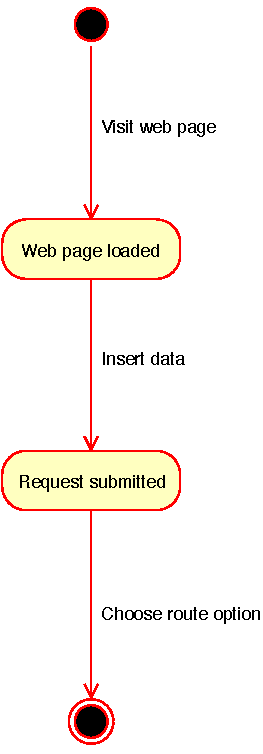
\includegraphics[scale=1]{Immagini/Automa_stati_finiti.pdf}}
\caption{Diagramma comportamentale}
\end{figure}
